%!TEX root = ../main.tex

\chapter{Kravspecifikation}

\begin{table}[H]
\centering
{\rowcolors{2}{white!80!black!30}{white!70!black!60} %farver på hver anden række -starter på 3
\setlength{\arrayrulewidth}{0.2mm}					 %tykkelse på linier 
\setlength{\tabcolsep}{10pt}						 %indryk i celle 
\renewcommand{\arraystretch}{1.5}					 %højden på tabelrum
\center
\begin{tabular}{|p{4cm}|p{4cm}|p{4cm}|}		 %længden på alle rum
\hline

\multicolumn{3}{|>{\columncolor{white!20!black!90}}m{13.44cm}|}{\textcolor{white}{\large{\textbf{Revision}}}} \\\hline
\rowcolor{white!70!black!60}
\textcolor{black}{\large{\textbf{Ændret af}}}&
\textcolor{black}{\large{\textbf{Version}}}&	
\textcolor{black}{\large{\textbf{Dato}}}\\
\hline
Alle	& 1	 	& 23-02-2015  \\
		& 		&   \\
		& 		&   \\
		& 	 	&   \\
\hline
\end{tabular}
}
\caption{Revision for kravspec}
\label{table:RevKrav}
\end{table}



%Aktører
\section{Aktører}
%!TEX root = ../../main.tex

I dette afsnit beskrives aktører og deres rolle i systemet. I figur \ref{photo:Aktor} ses aktørdiagram, som beskriver alle aktører og deres forhold til systemet


\begin{figure}[H]
	\centering
	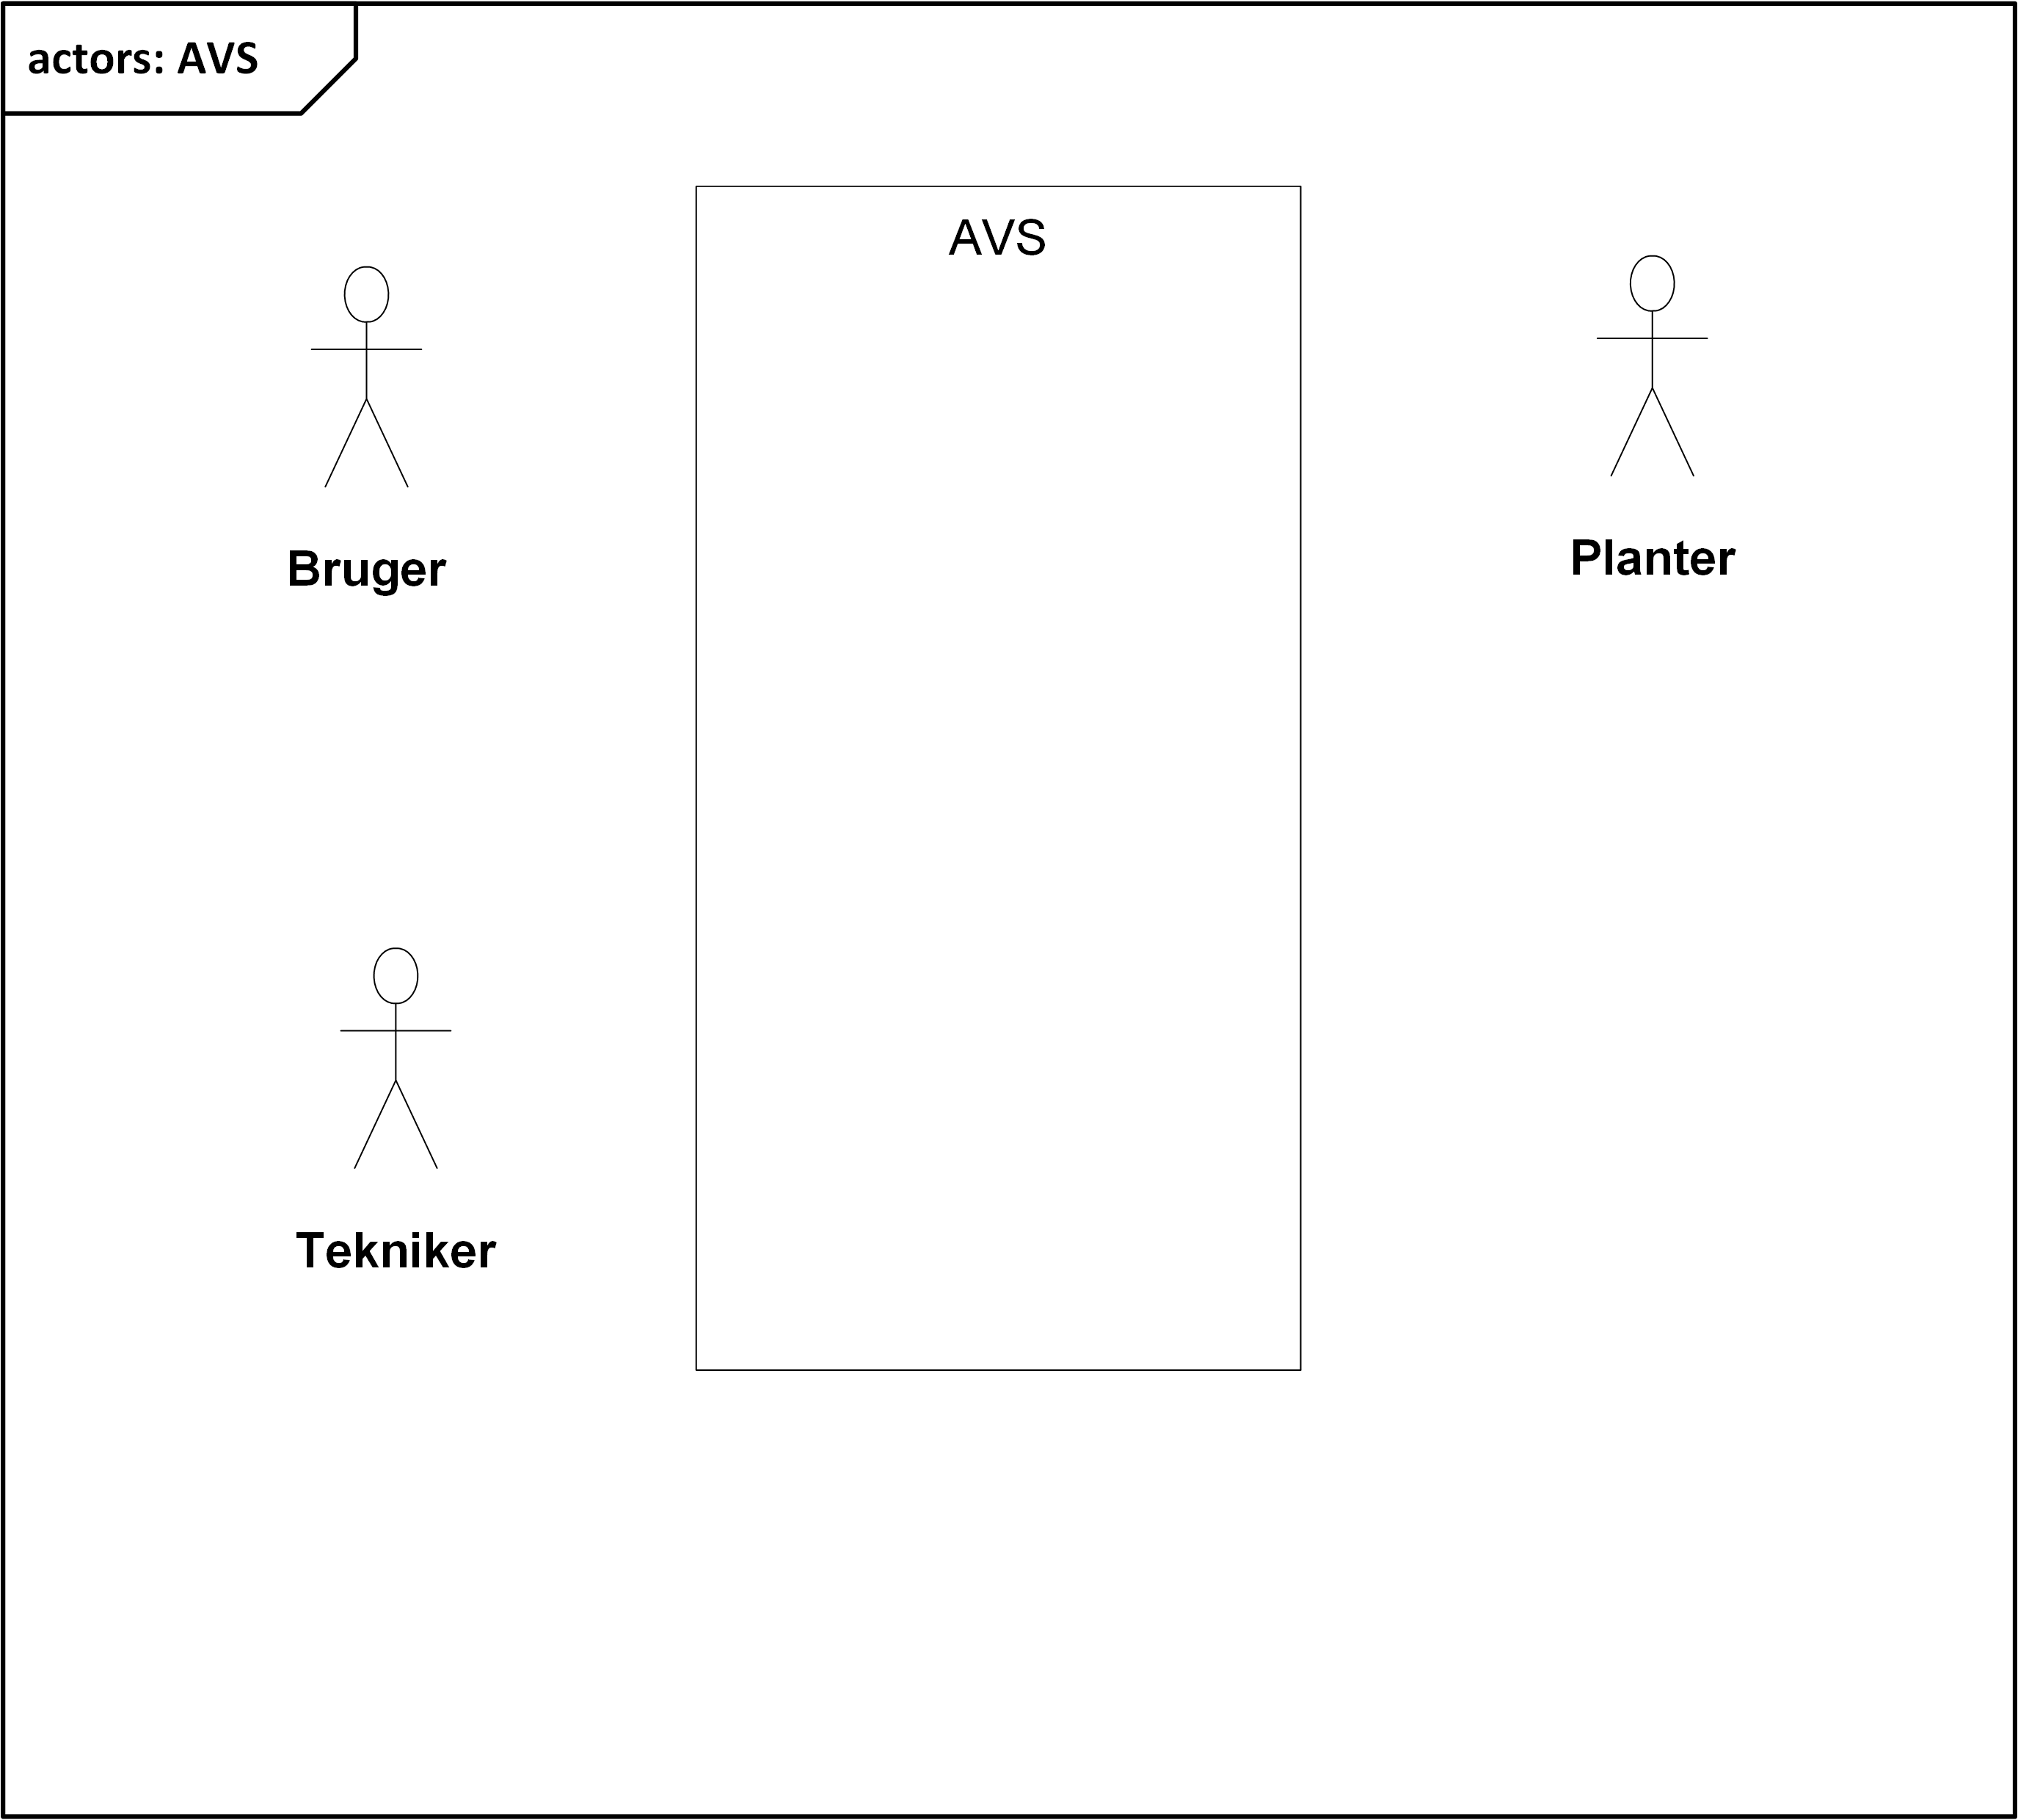
\includegraphics[scale=1]{Kravspecifikation/Actor/Photo/AVS_Actors}
	\caption{AVS Aktører}
	\label{photo:Aktor}
\end{figure}

\newpage

\subsection{Bruger}
\begin{usecase}
\addtitle{Aktørnavn}{Bruger} 
\addfield{type:}{Primær}
\addfield{Beskrivelse:}{Bruger er ham, som til dagligt tilgår systemet. Han ved hvor meget gødning og fugtighed planterne skal have, og angiver disse værdier i brugergrænsefladen. Det er brugeren som løbende ændrer værdierne, så systemet hele tiden er opdateret med værdier der passer til planternes vækststadier.}
\end{usecase}

\subsection{Tekniker}
\begin{usecase}
\addtitle{Aktørnavn}{Tekniker} 
\addfield{type:}{Primær}
\addfield{Beskrivelse:}{Tekniker er en specielt uddannet person. Han har den nødvendige viden om systemet til at kunne installere systemet fra opstart, opsætte nye vandkar mv. En Bruger kan også være tekniker.}
\end{usecase}






%Use Cases
\newpage
\section{Use Cases}
%	#1 Aflæs målinger
\subsection{Usecase 1}
Beskrivelse af denne use case
\begin{usecase}

\addtitle{Use Case 1}{Aflæs målinger} 

\addfield{Goal:}{mål!}

\additemizedfield{Initiatet by:}{
	\item bruger
	\item noget
}

\addfield{Actors:}{End-User}

\addfield{Concurrent occurances:}{1}

%Preconditions: What must be true on start and worth telling the reader?
\addfield{Preconditions:}{}

%Postconditions: What must be true on successful completion and worth telling the reader
\addfield{Postconditions:}{}

%Main Success Scenario: A typical, unconditional happy path scenario of success.
\addscenario{Main Success Scenario:}{
	\item The first action
	\item The second action
}

%Extensions: Alternate scenarios of success or failure.
\addscenario{Extensions:}{
	\item[2.a] Invalid login data:
		\begin{enumerate}
		\item[1.] System shows failure message
		\item[2.] User returns to step 1
		\end{enumerate}
	\item[5.a] Invalid subsriber data:
		\begin{enumerate}
		\item[1.] System shows failure message
		\item[2.] User returns to step 2 and corrects the errors
		\end{enumerate}
}


\end{usecase}

%	#2 Indtast data
\newpage
\subsection{Use case 2}
I denne use case ønsker brugeren at tilføre vand manuelt til planterne. Denne use case kan kun tilgås af en person. For at denne use case kan gennemføres skal der være vand i det kar der ønskes at vande fra samt at dette er tilføjet til systemet. Karet skal være koblet på mindst en sensor ø.
\begin{usecase}

\addtitle{Use Case 2}{Manuel vanding} 

\addfield{Mål:}{At tilføre vand til planterne}

\additemizedfield{Initieret af:}{
	\item Bruger
}

\addfield{Aktør:}{Bruger}

\addfield{Samtidige forekomster:}{1}

%Preconditions: What must be true on start and worth telling the reader?
\addfield{Prækondition:}{Der skal være vand i det kar der ønskes at vande fra og der skal være tilkoblet mindst en sonsor ø. GUI'en befinder sig i hovedmenuen}

%Postconditions: What must be true on successful completion and worth telling the reader
\addfield{Postkonditions:}{Der er vand ved planterne}

%Main Success Scenario: A typical, unconditional happy path scenario of success.
\addscenario{Hovedscenario:}{
	\item Bruger trykker på "Kar X" i GUI
	\item Systemet viser et skærmbillede hvor der kan vælges manuel vanding
	\item Bruger trykker på "Manuel vanding"
	\item Systemet begynder at vande
	\item Systemet ændre knappen for manuel vanding til stop maunel vanding
	\item[ ] [Ex.1 Karret er tomt]
	\item Når der ikke ønskes at vande længere trykker bruger på "Stop manuel vanding"
	\item Systemet stopper med at vande
}

%Extensions: Alternate scenarios of success or failure.
\addscenario{Udvidelser:}{
	\item[Ex.1] Karret er tomt:
		\begin{enumerate}
		\item[1.] Systemet stopper med at vande
		\end{enumerate}
}


\end{usecase}

%	#3 Manuel vanding
\newpage
\subsection{Use case 3}
I denne use case ønsker brugeren at tilføre vand manuelt til planterne. Denne use case kan kun tilgås en person, der der kun er en interface. For at denne use case kan gennemløbes skal der være vand i det kar der ønskes at vandes fra og der er indtastet systemdata som blev indtastet i use case 2.
\begin{usecase}

\addtitle{Use Case 3}{Manuel vanding} 

\addfield{Mål:}{At tilføre planterne vand}

\additemizedfield{Initieret af:}{
	\item Bruger
}

\addfield{Aktør:}{Bruger}

\addfield{Samtidige forekomster:}{1-Antal \gls{vandkar}}

%Preconditions: What must be true on start and worth telling the reader?
\addfield{Prækondition:}{Der skal være vand i det kar der ønskes at vande fra. Der er indtastet system data fra UC2.}

%Postconditions: What must be true on successful completion and worth telling the reader
\addfield{Postkonditions:}{Der er vand ved planterne}

%Main Success Scenario: A typical, unconditional happy path scenario of success.
\addscenario{Hovedscenario:}{
	\item Bruger tilgår systemet via \glslink{gui}{gui'en}
	\item Bruger vælger i menuen "Manuel vanding".
	\item System tilføre vand til \glslink{plante}{planterne}
	\item System stopper når den ønskede fugtighed i \glslink{gromedie}{gromediet} er nået.
}

%Extensions: Alternate scenarios of success or failure.
%\addscenario{Extensions:}{

%}


\end{usecase}

%	#4 Karstyring
\newpage
\subsection{Use case 4}
I denne use case vil brugeren indtaste volumen på karret for at systemet kan vide hvor meget gødning, der skal doseres. Der kan også ændres på volumen i perioder, hvor der bruges lidt vand, for at undgå vandet bliver dårligt. For at use casen kan gennemføres skal teknikeren have oprettet et kar, som er tilkoblet systemet.
\begin{usecase}

\addtitle{Use Case 4}{Indtast volumen} 

\additemizedfield{Mål:}{
\item Indtaste volumen på et vandkar
}

\addfield{Initieret af:}{
	Bruger   
}

\additemizedfield{Aktører:}{\item Primær: Bruger}

\addfield{Samtidige forekomster:}{1}

%Preconditions: What must be true on start and worth telling the reader?
\addfield{Prækondition:}{Der er oprettet et kar i systemet og det er tilkoblet}

%Postconditions: What must be true on successful completion and worth telling the reader
\addfield{Postkondition:}{Systemet er opdateret med volumen på karret }

%Main Success Scenario: A typical, unconditional happy path scenario of success.
\addscenario{Hovedscenarie:}{
	\item Bruger trykker på "Kar X" i GUI
	\item Systemet viser et skærmbillede hvor det er muligt at indtaste en volumen
	\item Bruger trykker på "volumen"
	\item Systemet viser en cursor i skrivefeltet tilhørende
	      volumen
	\item Bruger indtaster en volumen i liter
	\item Bruger trykker på "Gem" 
	\item Systemet gemmer volumen
}

%Extensions: Alternate scenarios of success or failure.
%\addscenario{Udvidelser:}{
%	\item[Ex.1] Teknikeren ønsker kun at aflæse værdier:
%		\begin{enumerate}
%		\item[1.] Teknikeren trykker på "OK"
%		\end{enumerate}
%}


\end{usecase}


\section{Ikke Funktionelle Krav}
Brugervenlighed:
\begin{itemize}
	\item Skal være intuitivt og let at opererer for udefrakommende:
	Der forudsettes en fungerende standard PC med Windows inkl. Explore/Chrome	/Firefox som browser

	\item Systemet skal kunne tilgås igennem en normal webbrowser:
		Her menes Explorer / Google Chrome / Firefox
	\item Systemet skal kunne tilgås over lokalt netværk samt over www
		Her forudsættes en fungerende internetopkoling og evt. lokalt netværk
\end{itemize}

Systembetingelser:
\begin{itemize}
	\item Systemet skal kunne fungere stabilt i temperaturintervallet (1 - 45grader Celsius)
	\item Systemet skal kunne fungere stabilt under høj luftfugtighed (op til 50%)
	\item Systemet skal være let at vedligeholde på daglig basis
		Systemets reservedele skal være lette at udskifte og skaffe.
\end{itemize}

Ydelse:
\begin{itemize}
	\item Systemet skal kunne fylde vandkarret på max. 2 min.
	\item Systemet skal kunne tømme vandkarret på max. 2 min.
	\item Systemet skal kunne dosere vand til gromediet med min 0,5 / max 2 liter/min.
	\item Systemet skal kunne dosere gødning til karret på max. 30 sek.
\end{itemize}
%Kravspecifikation